The convolution operation is a combination of concepts from the fcl and pooling.
Like in pooling, values get aggregated from inside a specific region of influence.
They do however not get treated uniformly, but scaled with (learnable) weights before being summed up.

The comparison between a \emph{normal convolution}, a \emph{depthwise convolution} and a \emph{depthwise separable convolution} is given in \autoref{fig:comparison-depthwise-convolution}.

\begin{figure}[htbp]
    \centering
    \makebox[\textwidth][c]{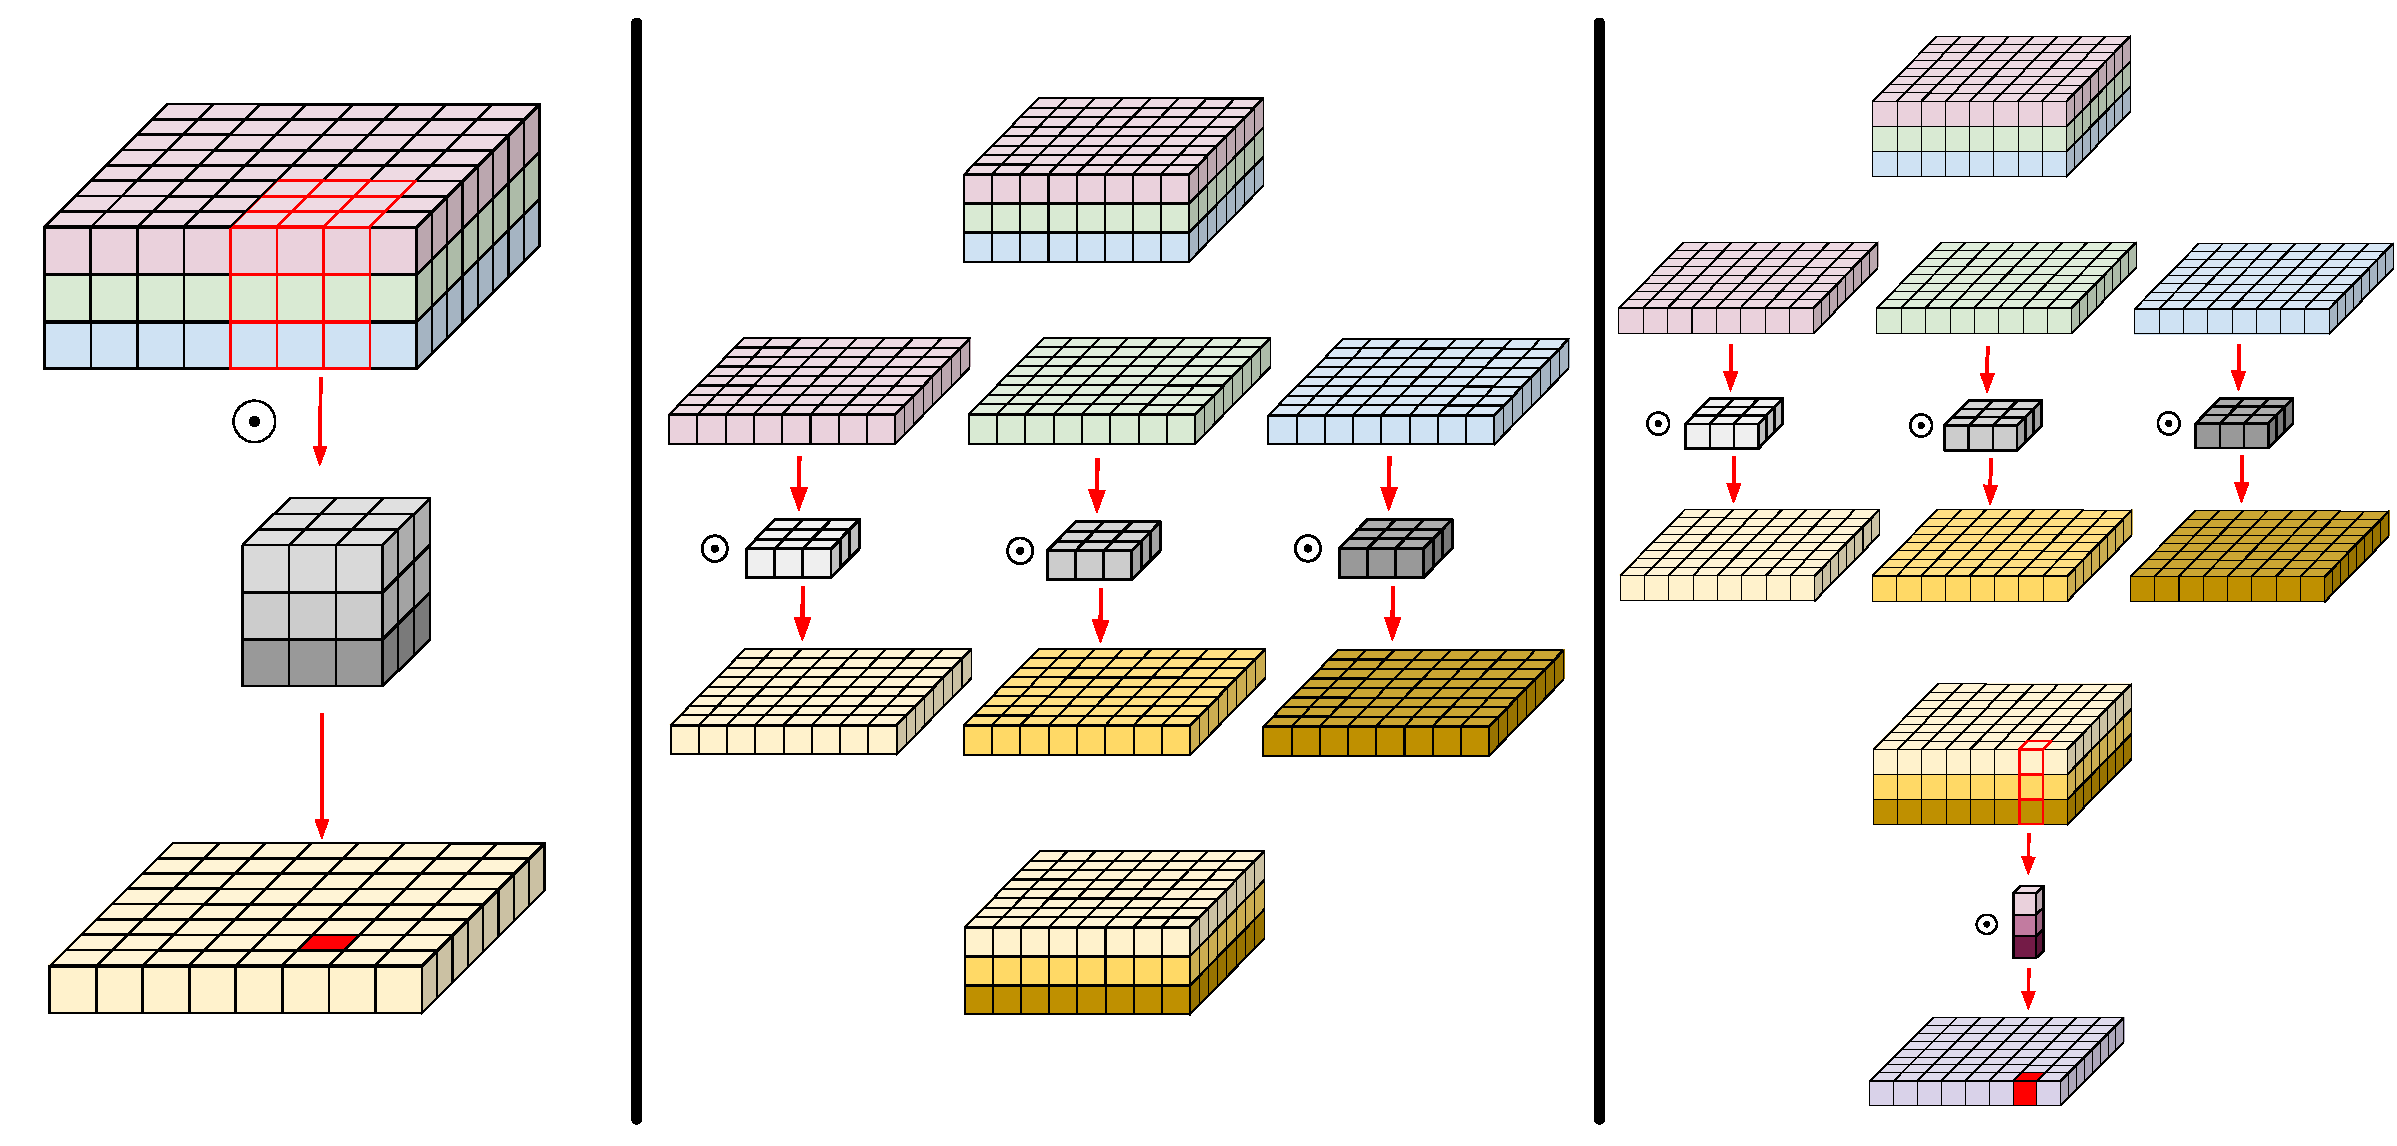
\includegraphics[width=1.1\textwidth]{./architectures/theory/convolutions/depthwise.pdf}}
    \caption{This figure show the differences between a \emph{normal convolution} (left), a \emph{depthwise convolution}  (middle) and a \emph{depthwise separable convolution} (right).
    The normal convolution has a 3D-kernel. The depthwise convolution splits this into multiple 2D-kernels.
    The depthwise separable convolution works basically in the same way as the depthwise, but at the end a 1D-kernel (1$\times$1-convolution) is used to combine the channels.
     Original image from \cite{separableConvolutions}, but modified and almost completely redrawn.}
    \label{fig:comparison-depthwise-convolution}
\end{figure}



The implementation of the symmetric depthwise convolution for images can be found at \cite{selfComputerScience}, \filepath{/models/helpers/SymmConv2d.py}.


% - focus on differences between depthwise and normal convolution
% - symmetrical convolutions with shared weights and their implementation 

% SOURCE: \cite{mobileNetPaper}
% - reduce network size and costs to be able to ship for low power/storage mobile devices

% SOURCE: \cite{channelNets}
% - citation on different styles of convolution channel usage
% - even improves upon depthwise separable convolutions 

% SOURCE: \cite{symmetricConvolutionImplementation}
% - symmetric convolutions

% SOURCE: \cite{backpropagationInConvolutions}
% - because of missing backpropagation
